\chapter{PROCEDURE} \label{ch:procedure}
\subsection{Setup and Initialization}
\begin{enumerate}
    \item Four columns were created using sticky notes as headers: \textbf{To Do}, \textbf{Doing}, \textbf{Test}, and \textbf{Done}
    \item Each of the nine tasks was written on individual sticky notes and placed in the \textit{To Do} column
    \item Team members reviewed all tasks and discussed initial assignments
    \item Photographic documentation began with the initial board state (Figure \ref{fig: Board 1}
\end{enumerate}
\begin{figure}[H]
    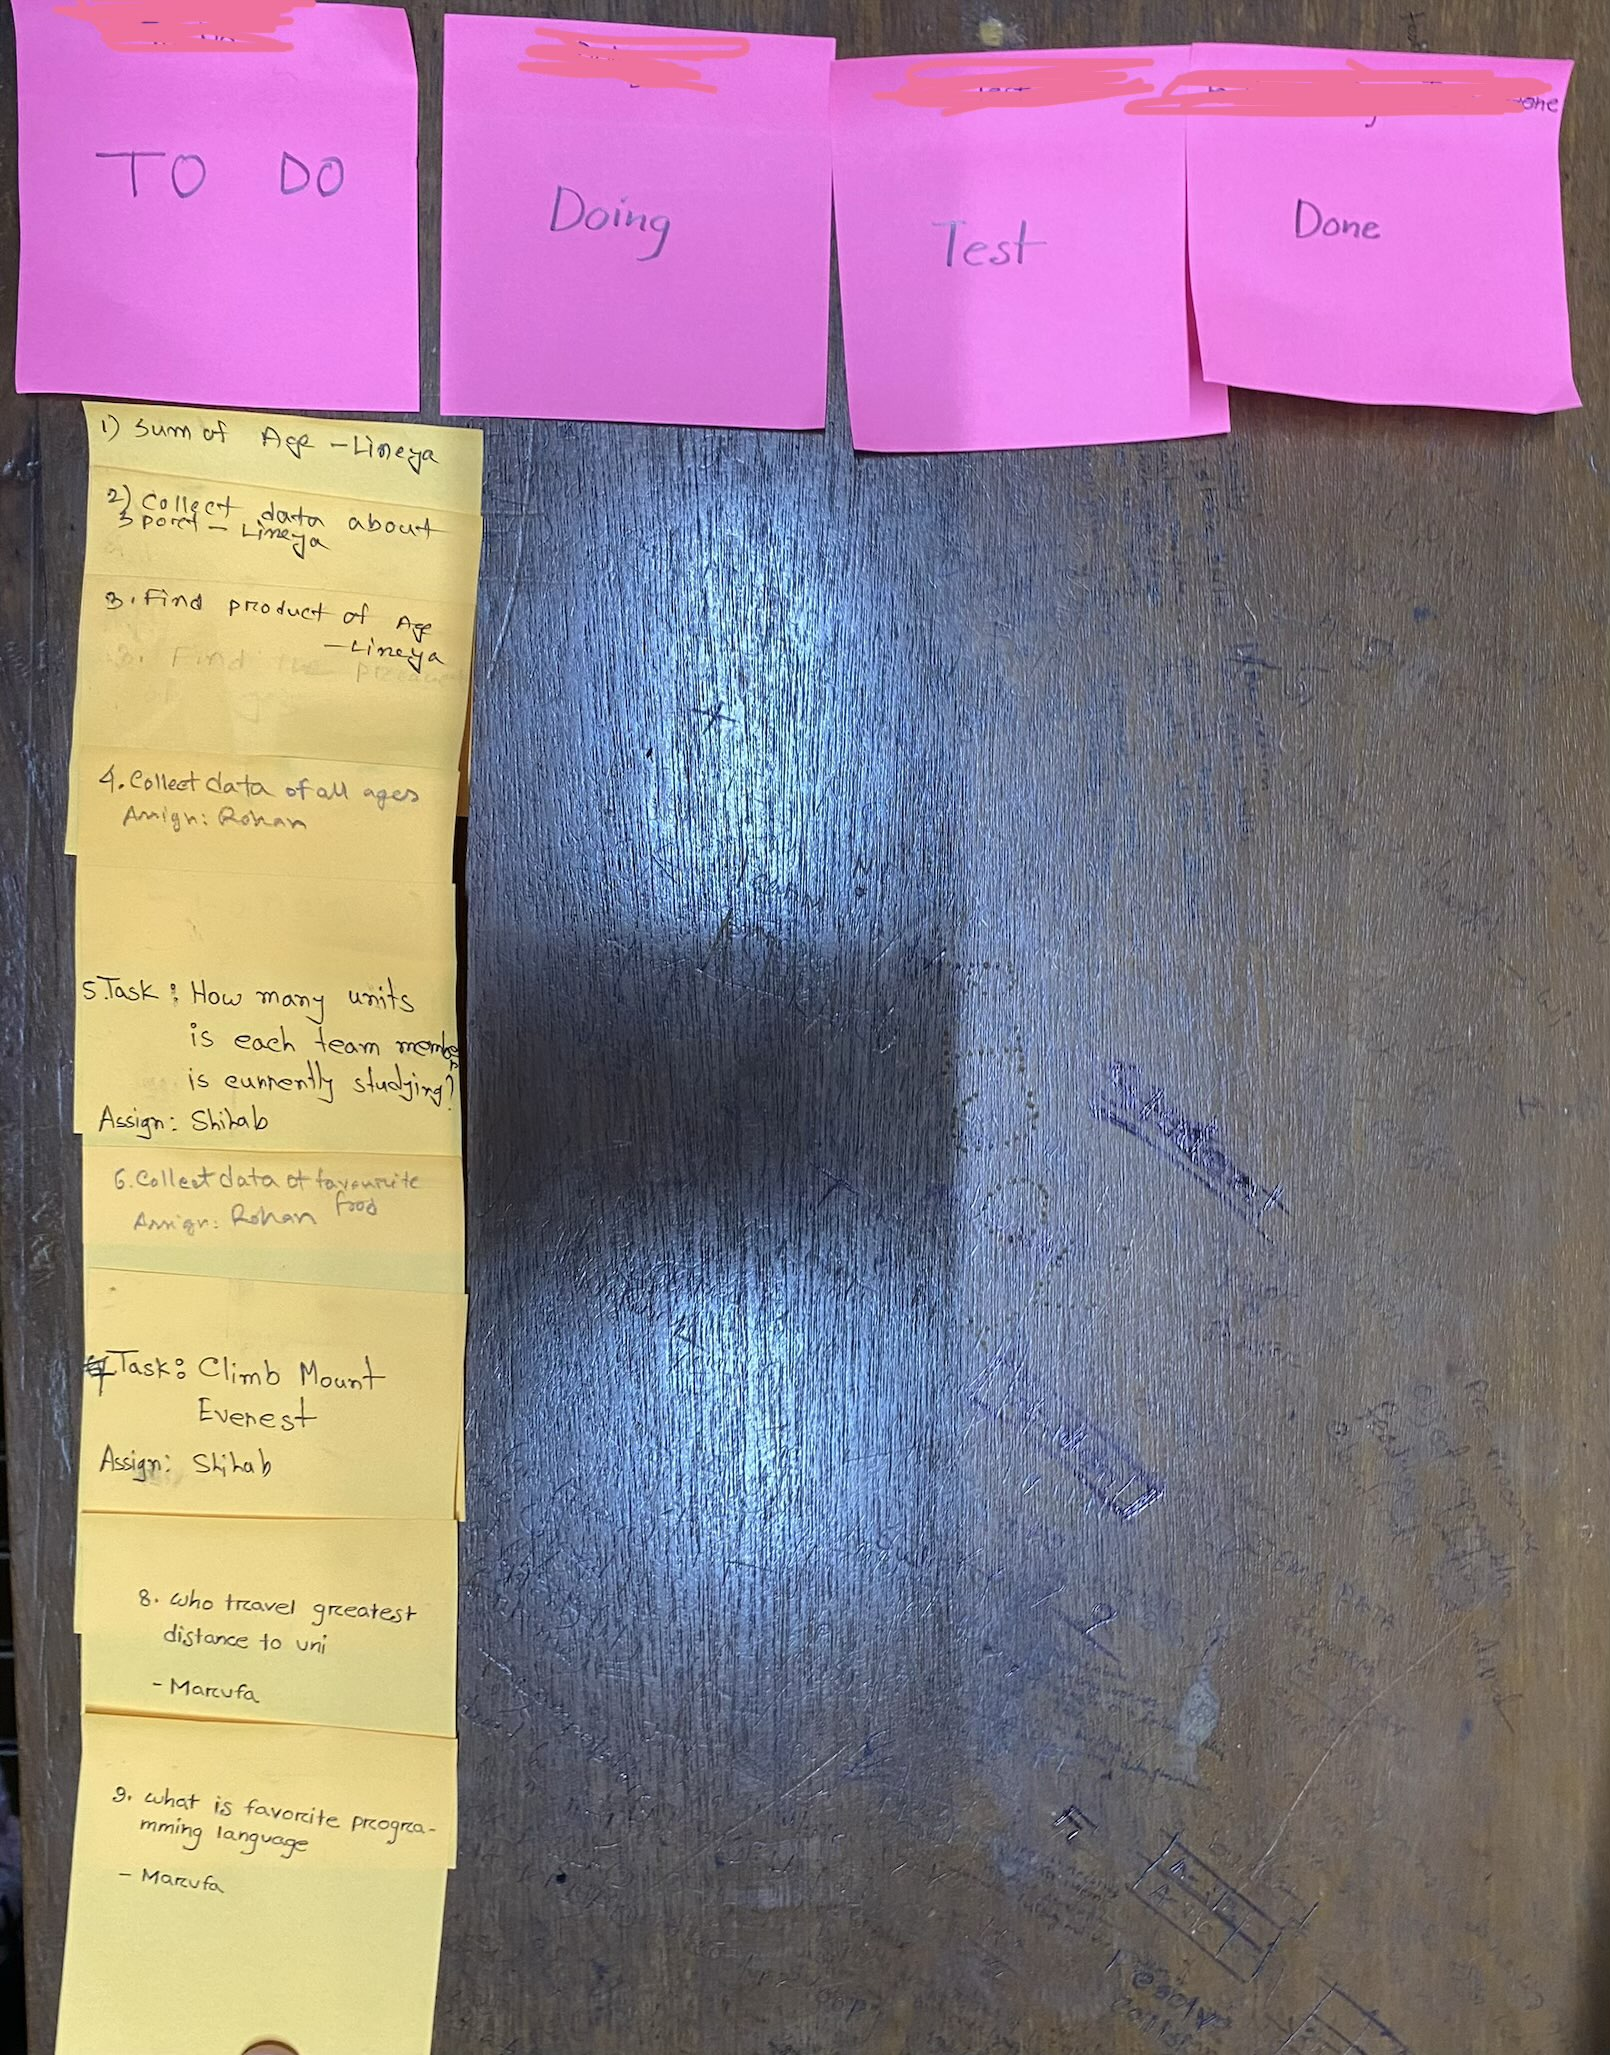
\includegraphics[width=0.5\textwidth]{figures/1.jpg}
    \label{fig: Board 1}
\end{figure}

\subsection{Task List and Assignments}
The following tasks were assigned during the exercise:
\begin{enumerate}
    \item Find the sum of all team members' ages. (Assigned to: Lineya)
    \item Collect data about sports each member likes. (Assigned to: Lineya)
    \item Find the product of all team members' ages. (Assigned to: Lineya)
    \item Collect data about the age of each member. (Assigned to: Rohan)
    \item How many units is each team member currently studying? (Assigned to: Shihab)
    \item Collect data about favorite food of each member. (Assigned to: Rohan)
    \item Climb Mount Everest. (Assigned to: Shihab)
    \item Who travels the greatest distance to university? (Assigned to: Marufa)
    \item What is the favorite programming language of the team? (Assigned to: Marufa)
\end{enumerate}
\begin{figure}[H]
    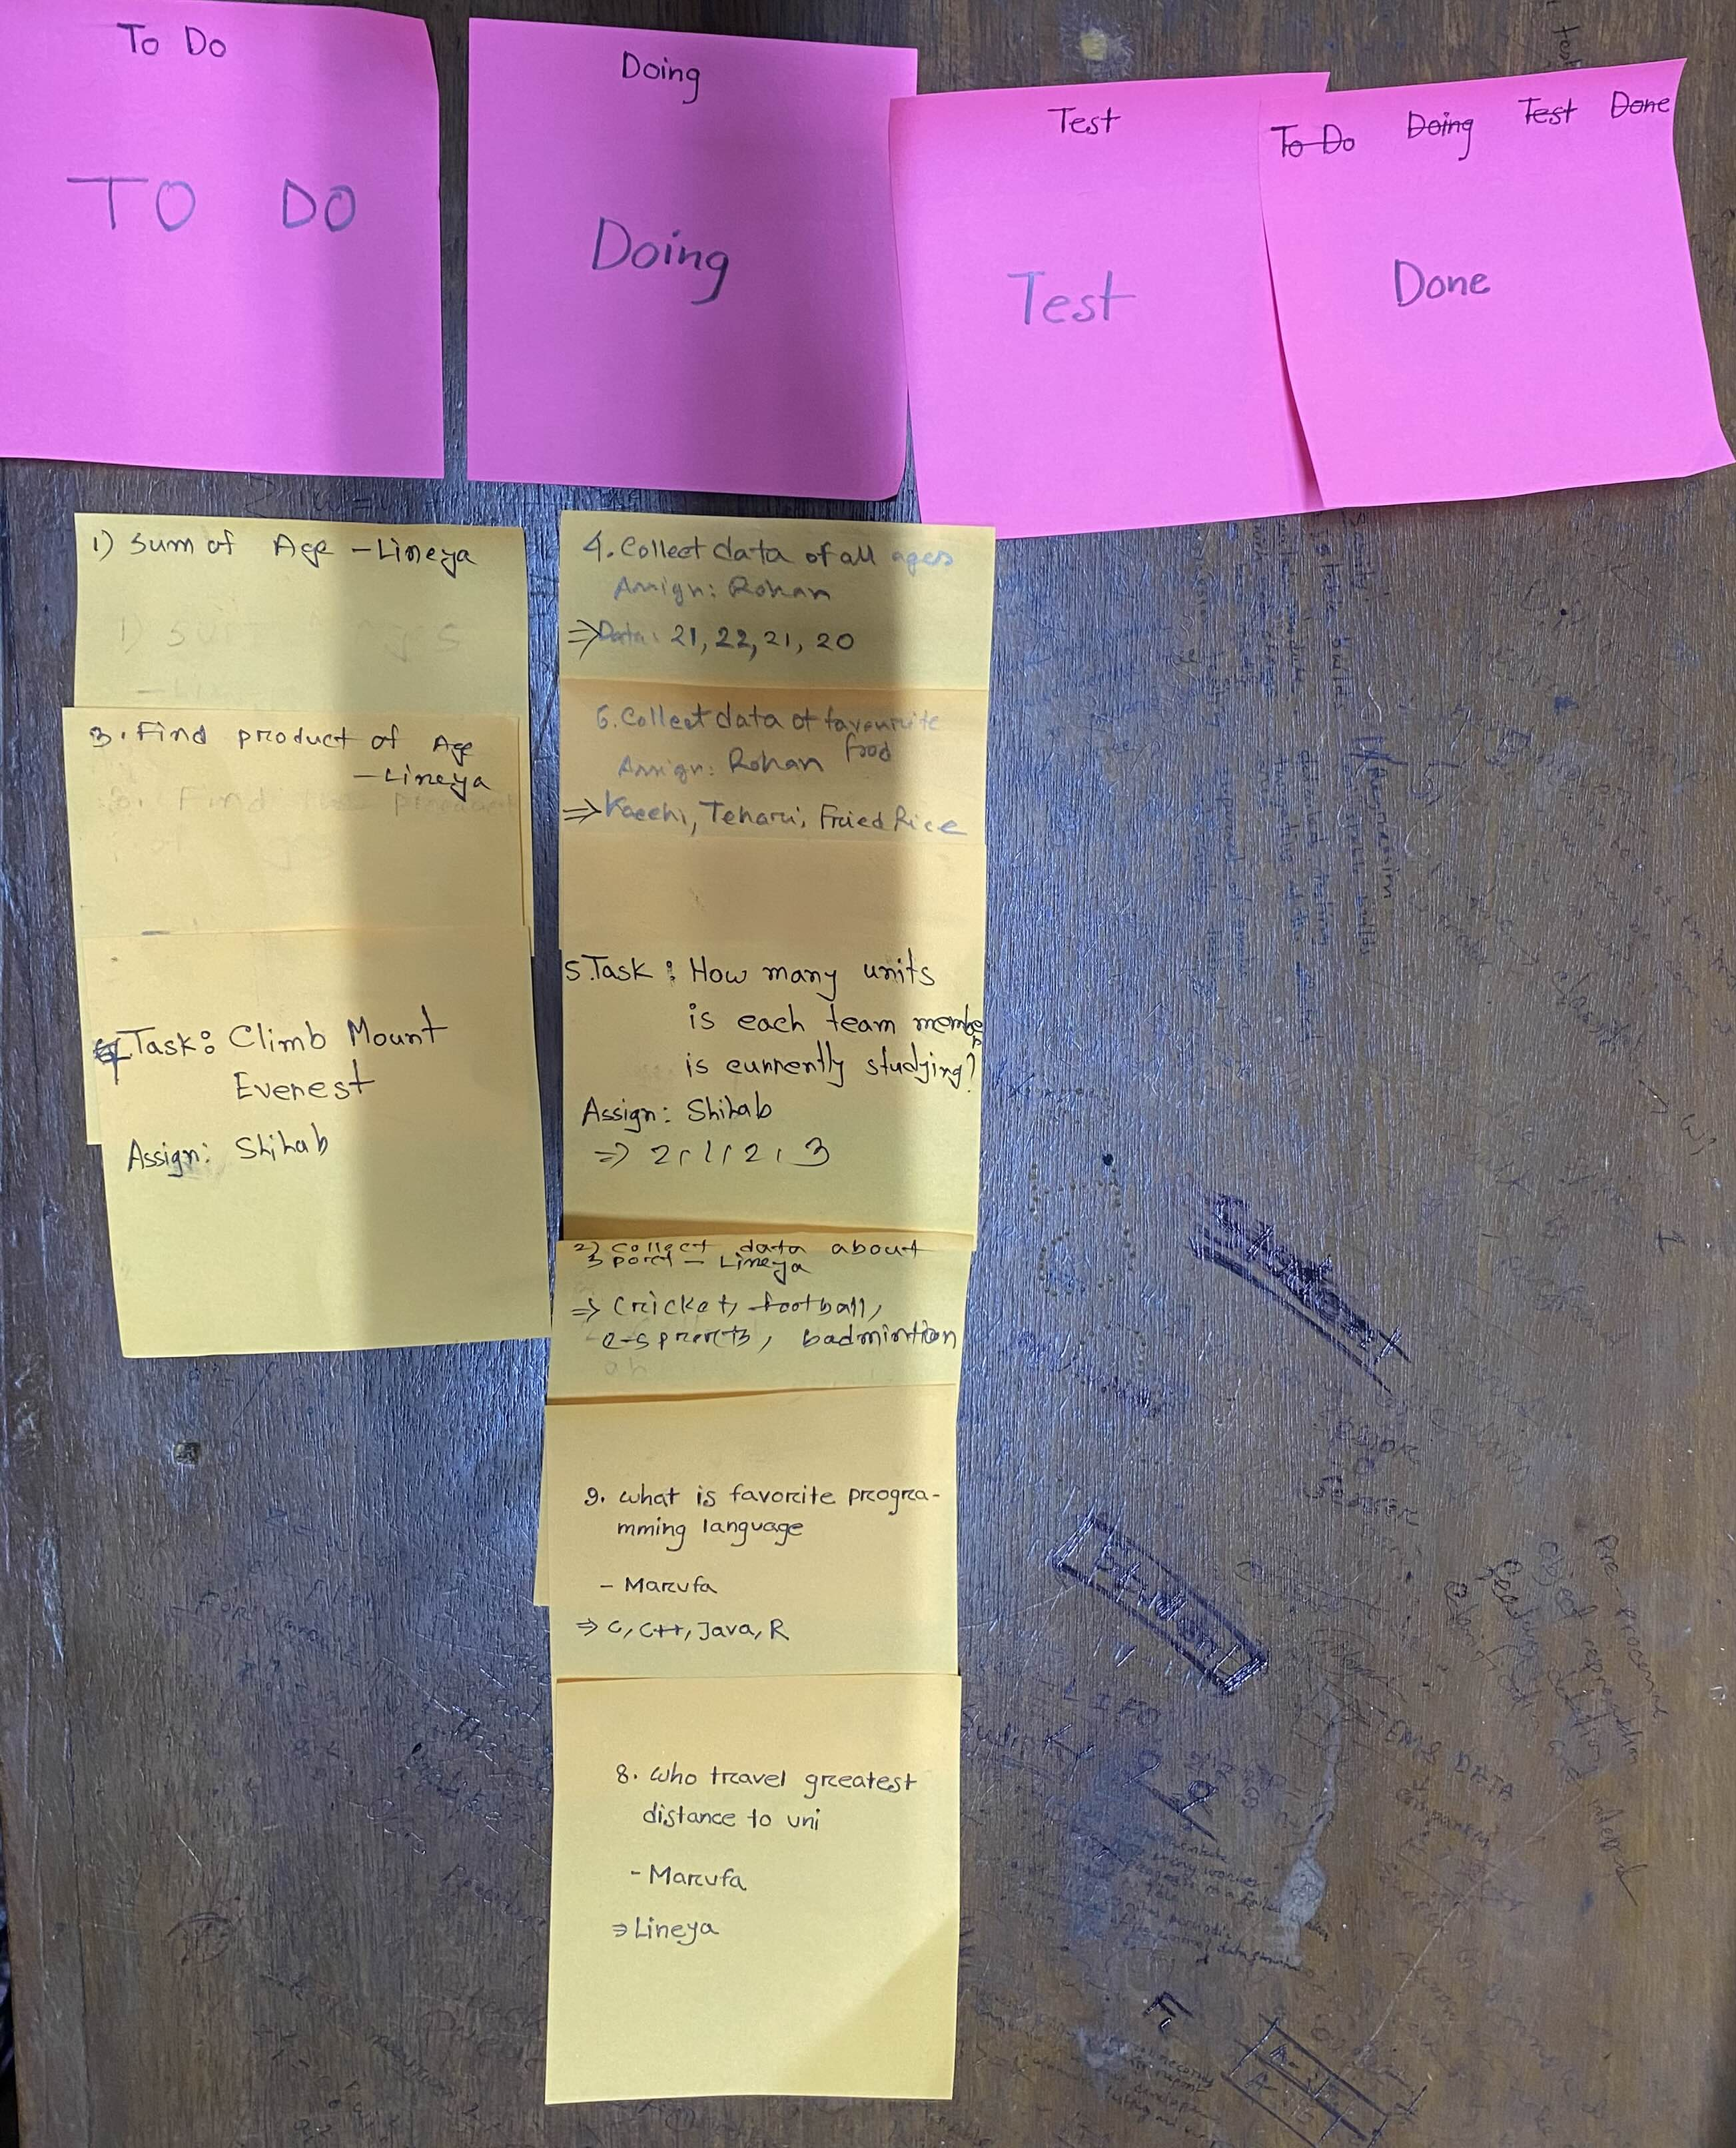
\includegraphics[width=0.5\textwidth]{figures/2.jpg}
    \label{fig: Board 2}
\end{figure}
\begin{figure}[H]
    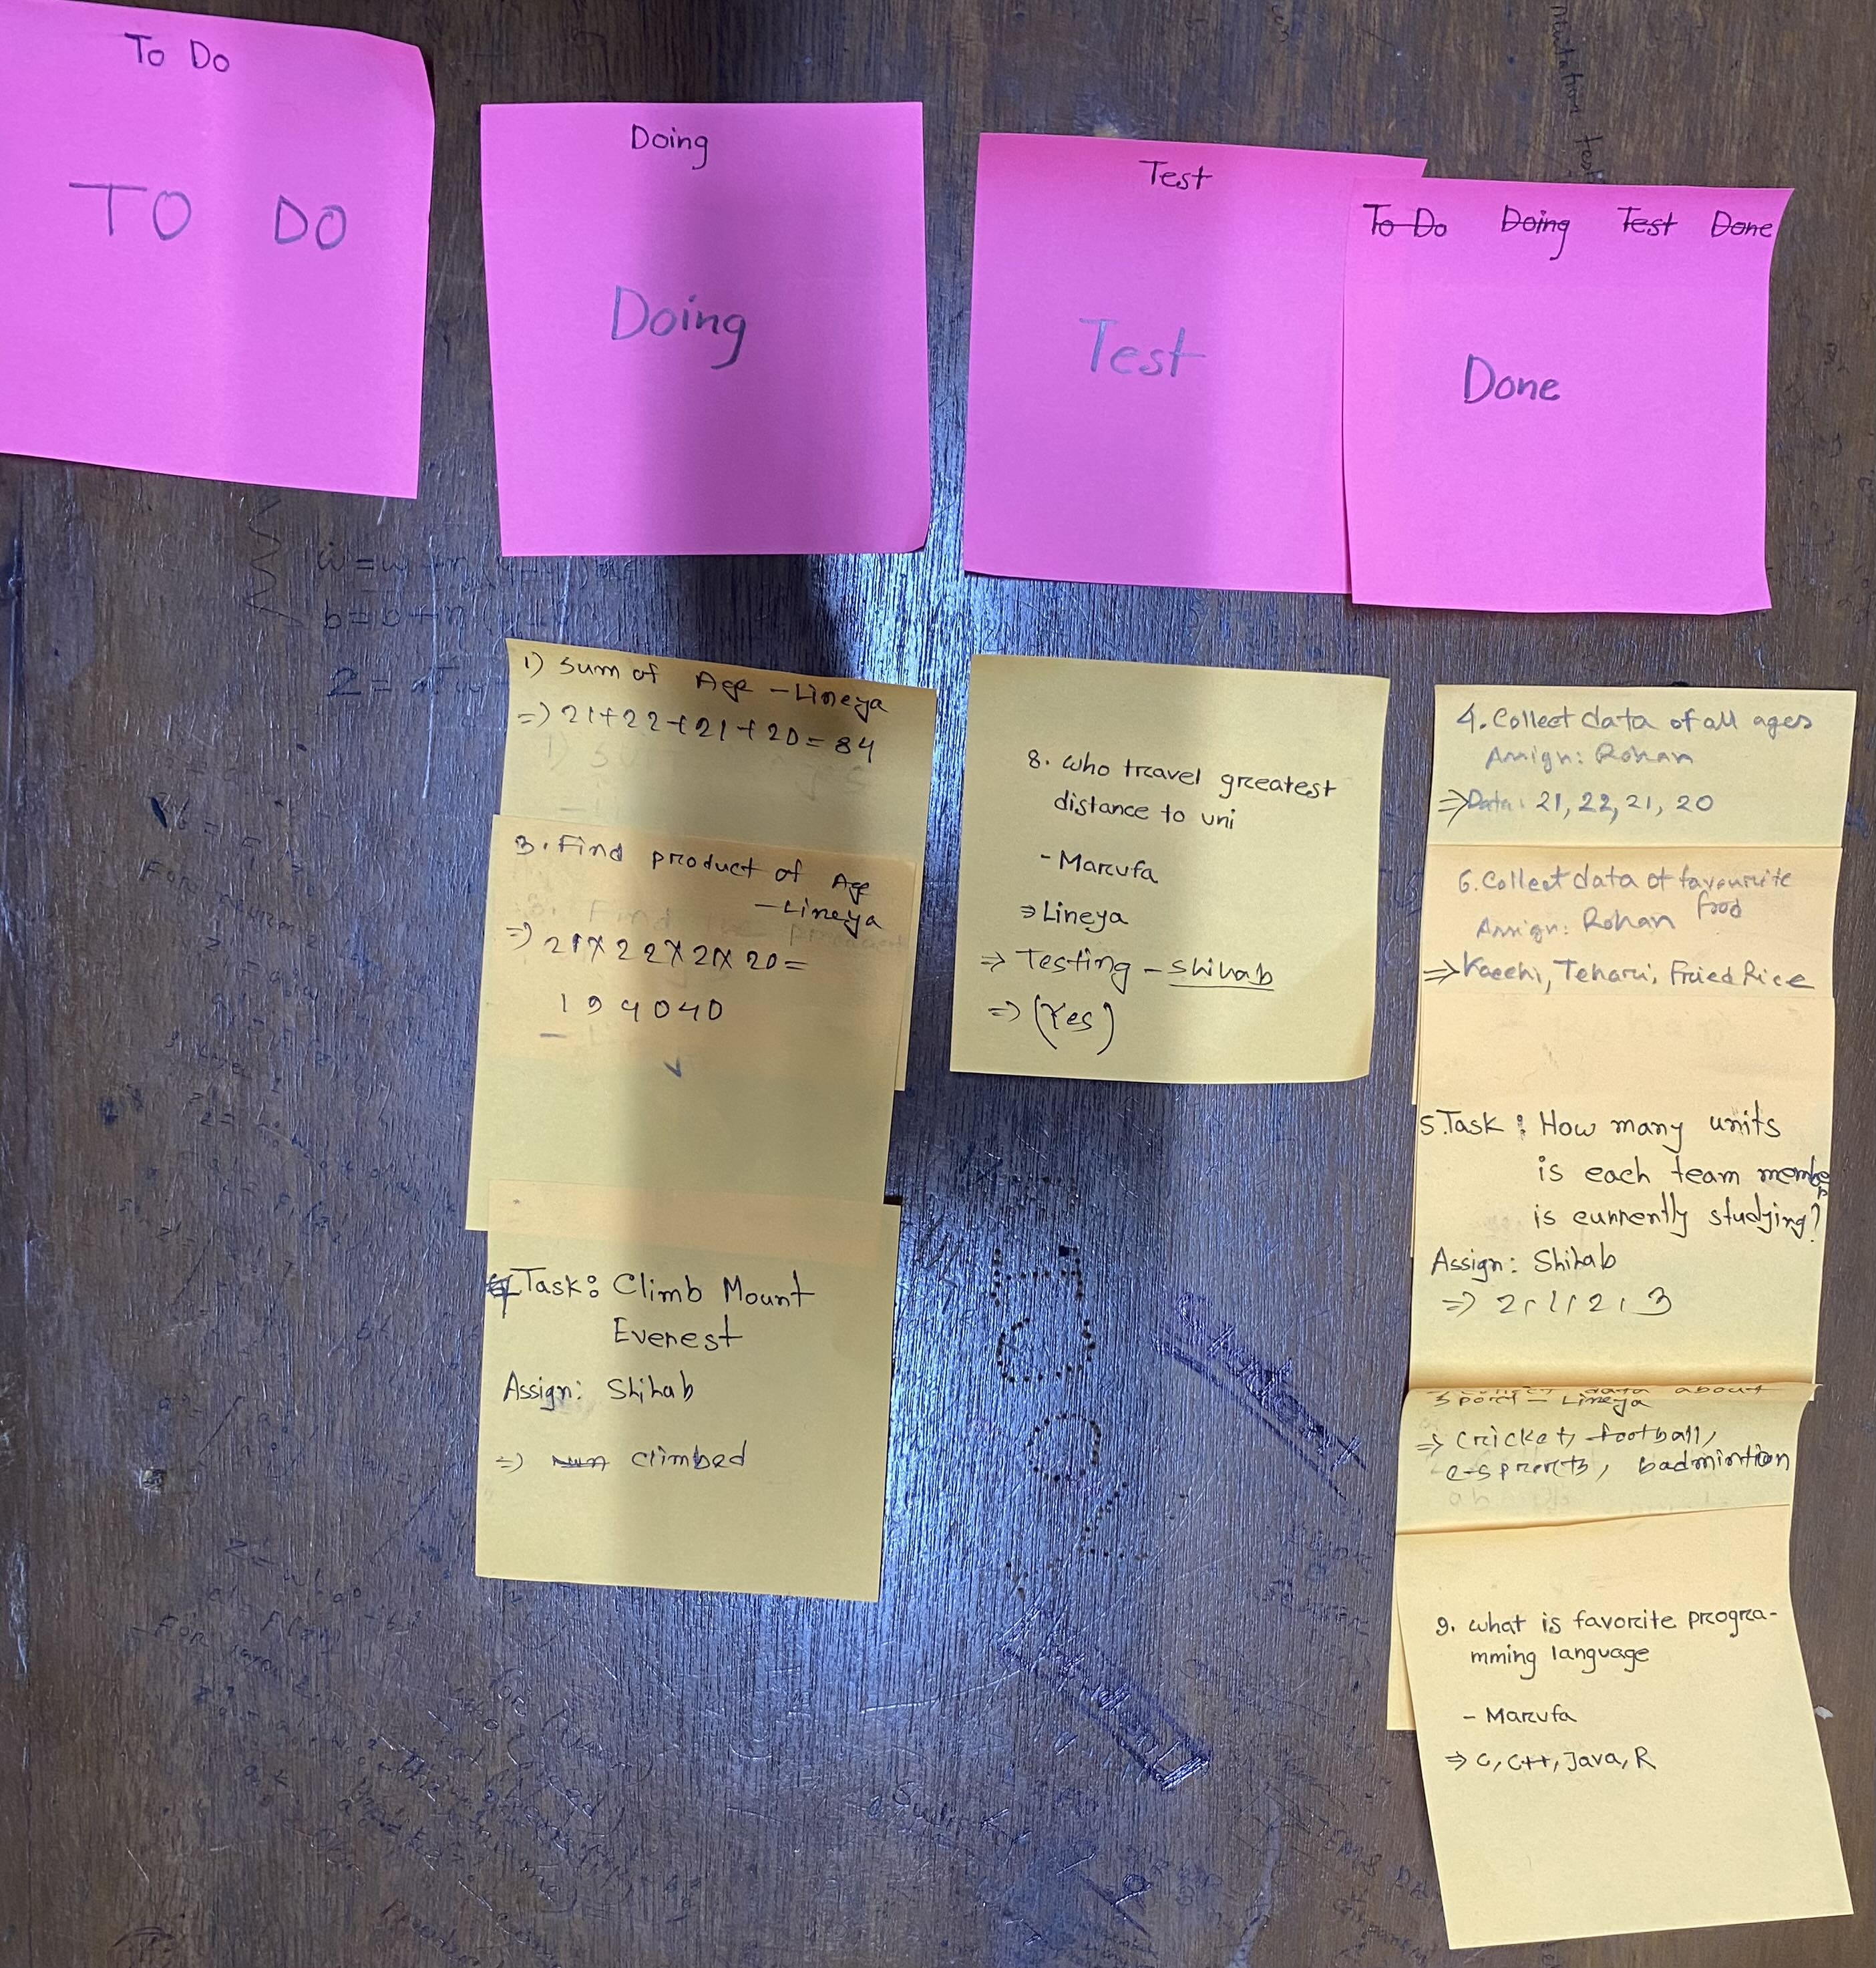
\includegraphics[width=0.5\textwidth]{figures/3.jpg}
    \label{fig: Board 3}
\end{figure}

\subsection{Execution Protocol}
\begin{itemize}
    \item Team members self-selected or were assigned tasks based on availability and preference
    \item When starting a task, the responsible member moved the sticky note from \textit{To Do} to \textit{Doing}
    \item Upon completion, calculation tasks moved to \textit{Test} for peer verification
    \item Non-calculation tasks moved directly to \textit{Done} after completion
    \item A different team member verified calculation tasks before final approval
    \item Photographs were taken at each significant board state change
    \item Parallel execution was encouraged for independent tasks
\end{itemize}
\begin{figure}[H]
    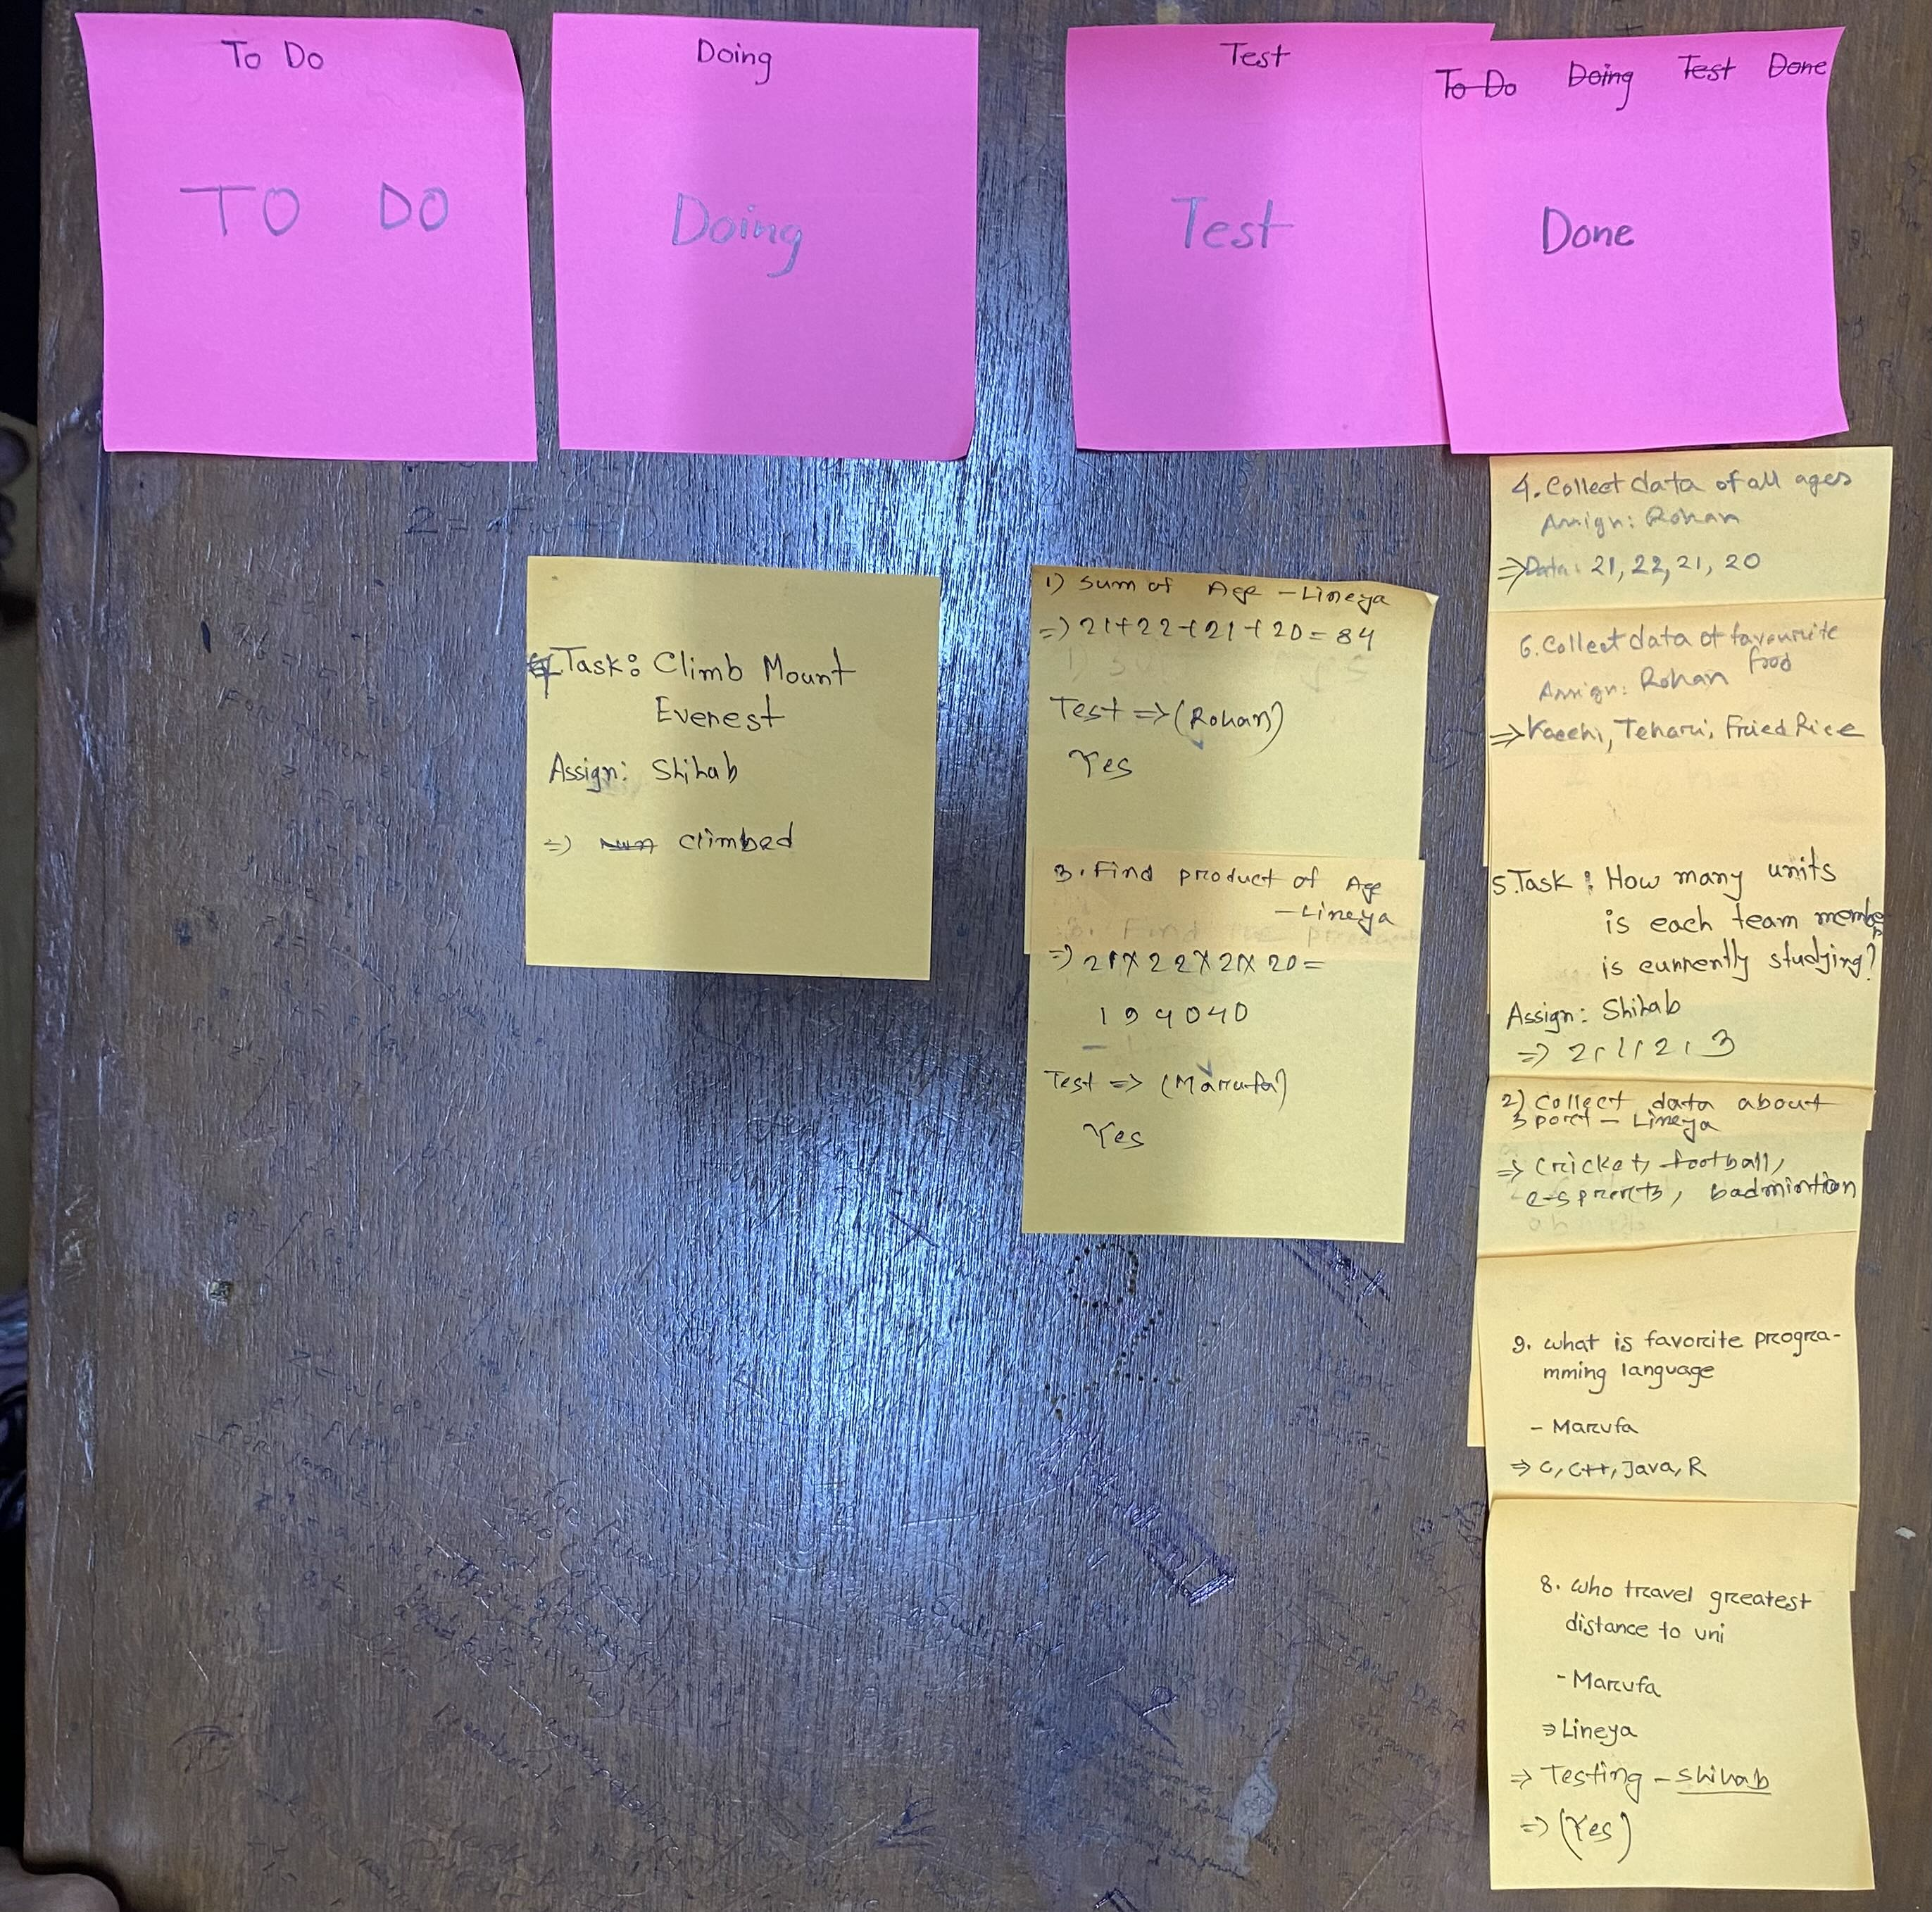
\includegraphics[width=0.5\textwidth]{figures/4.jpg}
    \label{fig: Board 4}
\end{figure}
\begin{figure}[H]
    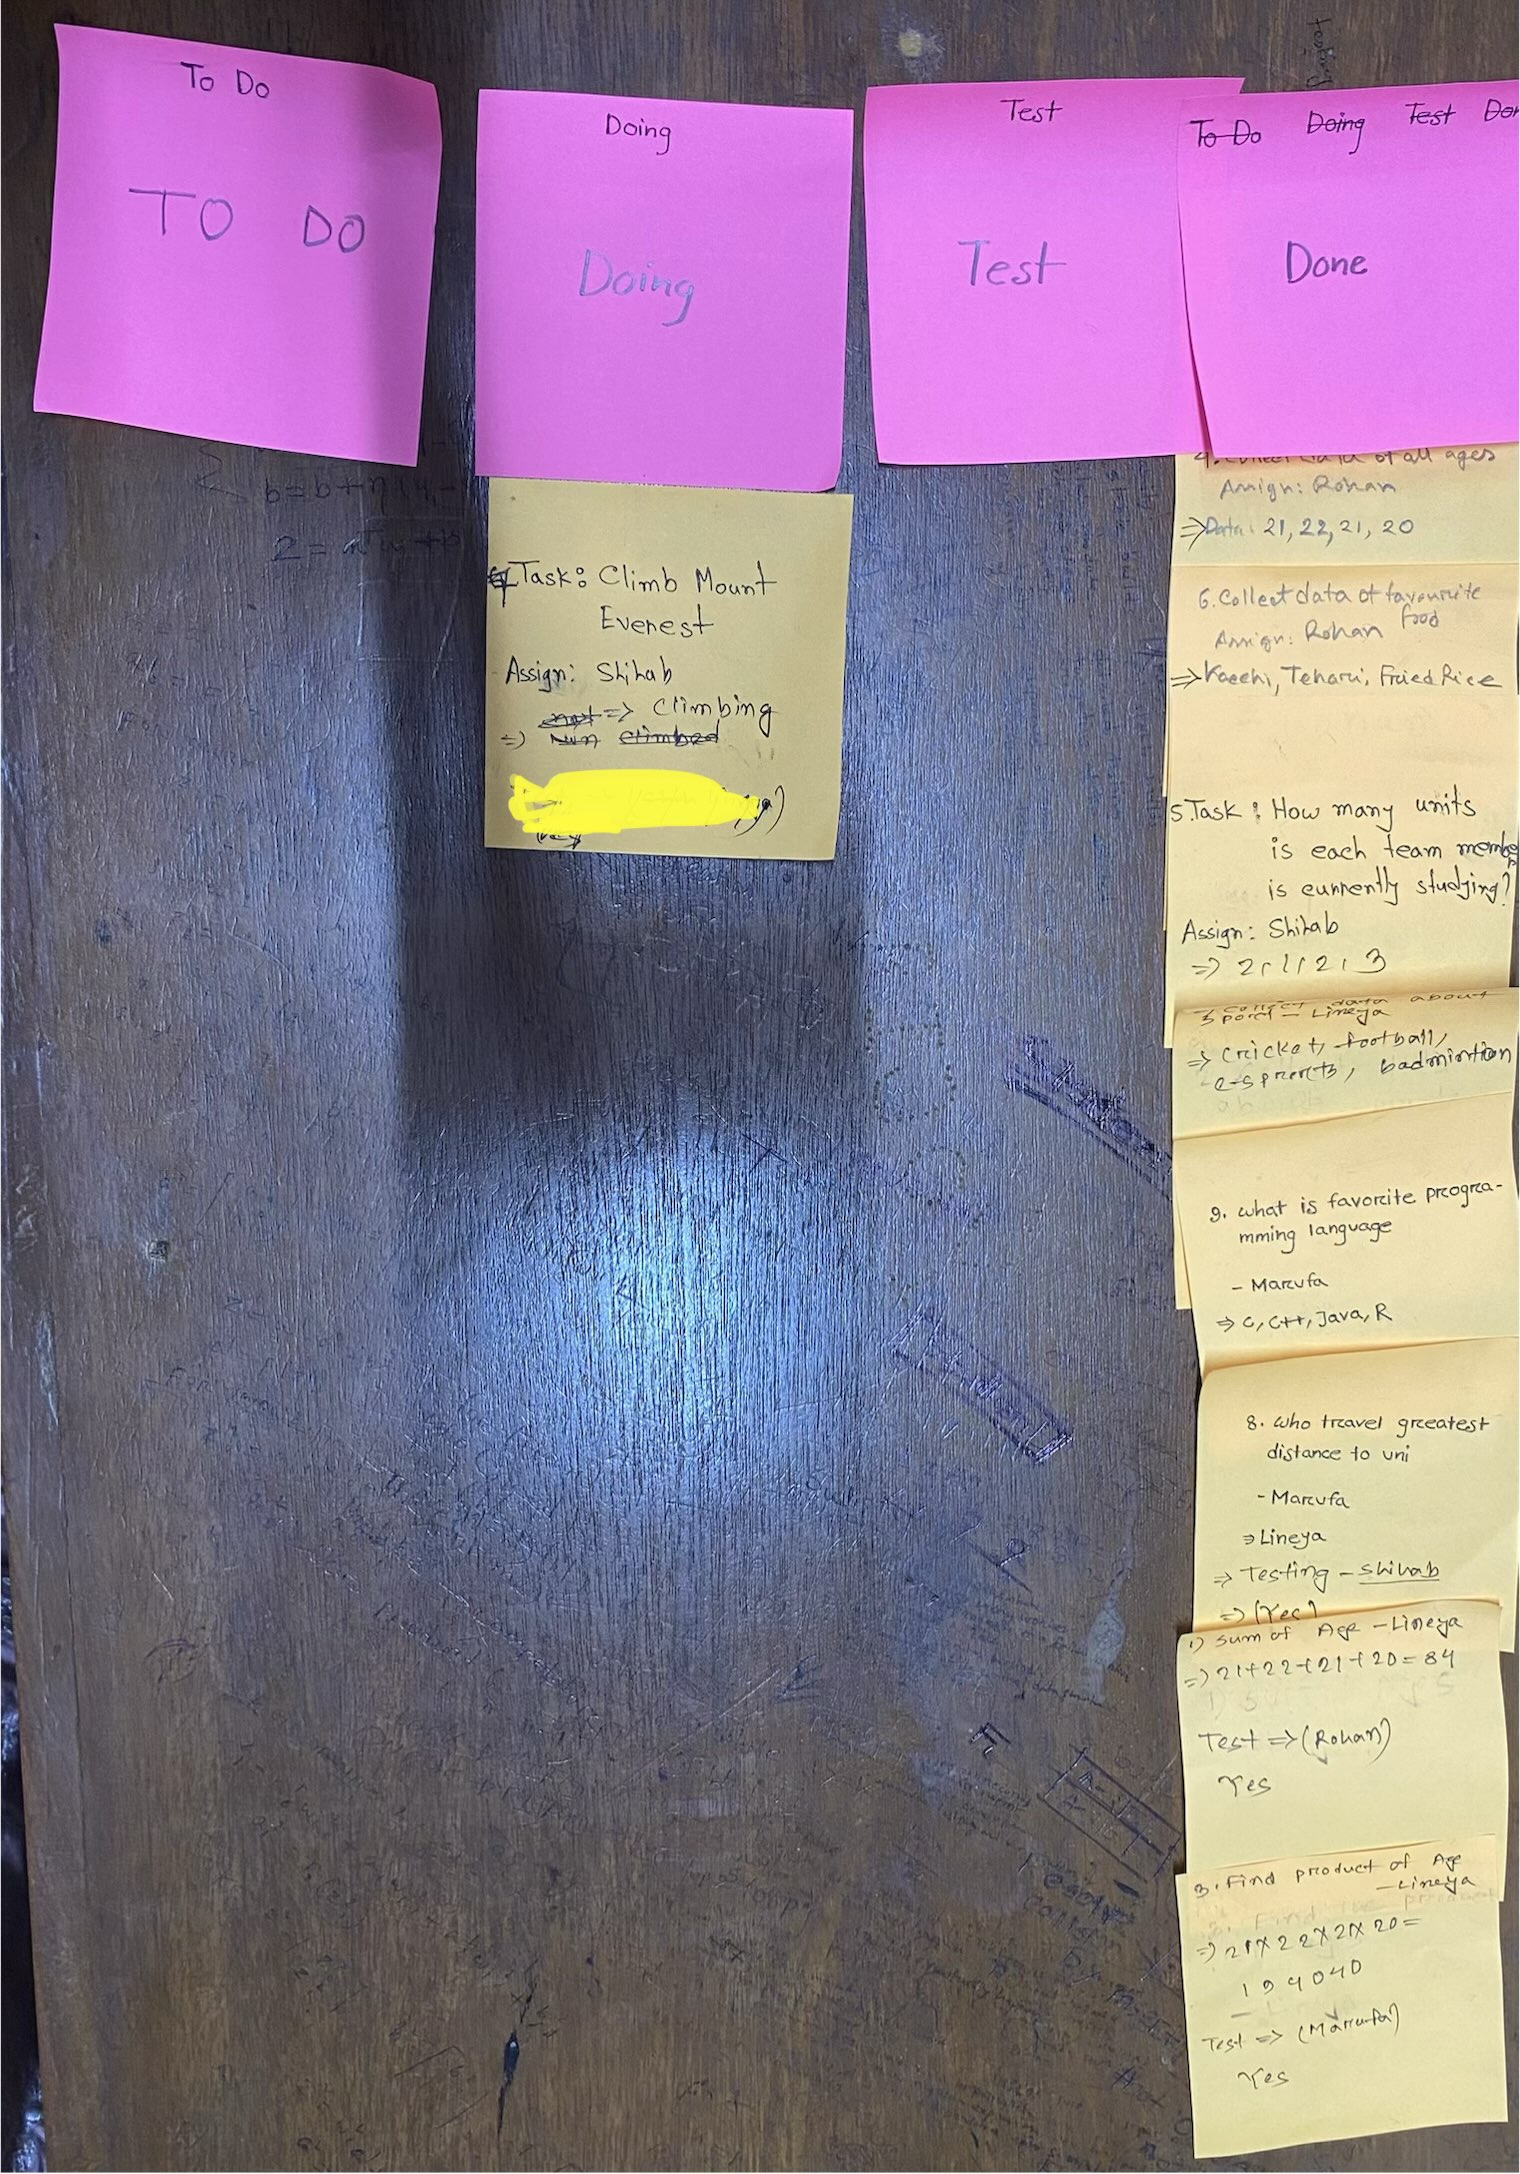
\includegraphics[width=0.5\textwidth]{figures/5.jpg}
    \label{fig: Board 5}
\end{figure}
